\documentclass[11pt]{article}
\usepackage[margin=1in]{geometry}
\usepackage{amsmath}
\usepackage{booktabs}
\usepackage{graphicx}
\usepackage{hyperref}
\usepackage{listings}
\usepackage{xcolor}
\usepackage{enumitem}

\lstset{
  basicstyle=\ttfamily\small,
  keywordstyle=\color{blue},
  commentstyle=\color{gray},
  breaklines=true,
  frame=single,
  numbers=left,
  numberstyle=\tiny\color{gray}
}

\title{Modernization Report:\\Floyd--Warshall CPU vs GPU Experiments}
\author{Kenneth Peter Fernandes\\Harrisburg University of Science and Technology\\CISC 719 -- IMC06\\Instructor: Prof. Majid Shaalan, Ph.D.}
\date{\today}

\begin{document}
\maketitle

% ============================================================
\section{Introduction}
% ============================================================

In this report, I describe the modernizations I made to the Floyd--Warshall reference implementations (R1 and R2), present the benchmark results from running all variants on Google Colab with a Tesla T4 GPU, and discuss what the results tell us about performance bottlenecks and future improvements.

The starting point was R2's Jupyter notebook, which provides a NumPy CPU baseline and a naive Numba CUDA kernel. I kept both of these as Variants 1 and 2, then added two new GPU implementations as modernizations:

\begin{itemize}
  \item \textbf{Variant 3 -- Tiled Numba CUDA kernel (32$\times$32 + shared memory):} A hand-written kernel that uses shared memory to cache row $k$ and column $k$ values, reducing redundant global memory reads.
  \item \textbf{Variant 4 -- CuPy broadcasting:} A high-level GPU implementation that mirrors the NumPy broadcasting approach but runs entirely on GPU memory using CuPy.
\end{itemize}

All four variants were tested on Google Colab (Tesla T4 GPU, 16 GB VRAM) at problem sizes $n = 256, 512, 1024,$ and $2048$. All GPU variants produced results identical to the CPU baseline (max absolute difference = 0.0 for all sizes), confirming correctness.

% ============================================================
\section{What Was Modernized}
% ============================================================

\subsection{Baseline Implementations (from R2)}

\textbf{Variant 1 -- NumPy CPU baseline.} This is the sequential implementation from R2 (cell 3). In our notebook (Cell 2, \texttt{floyd\_warshall\_cpu}), the core loop is:

\begin{lstlisting}[language=Python]
for k in range(num_nodes):
    dist_ik = dist[:, k][:, None]   # column k as (n, 1)
    dist_kj = dist[k, :][None, :]   # row k as (1, n)
    dist = np.minimum(dist, dist_ik + dist_kj)
\end{lstlisting}

For each intermediate node $k$, it extracts column $k$ and row $k$ as vectors and uses \texttt{np.minimum} with broadcasting to update the entire $n \times n$ matrix in one step. It runs on a single CPU core.

\textbf{Variant 2 -- Naive Numba CUDA kernel (16$\times$16).} This is the GPU baseline from R2 (cell 5), which mirrors the CUDA C++ kernel in R1 (lines 64--82). In our notebook (Cell 3, \texttt{naive\_floyd\_kernel}), the kernel is:

\begin{lstlisting}[language=Python]
@cuda.jit
def naive_floyd_kernel(dist_matrix, num_nodes, k):
    i, j = cuda.grid(2)
    if i < num_nodes and j < num_nodes:
        dist_i_to_k = dist_matrix[i, k]
        dist_k_to_j = dist_matrix[k, j]
        path_through_k = dist_i_to_k + dist_k_to_j
        if path_through_k < dist_matrix[i, j]:
            dist_matrix[i, j] = path_through_k
\end{lstlisting}

For each $k$-step, it launches a 2D grid of threads where each thread updates exactly one cell $(i, j)$. The block size is $16 \times 16 = 256$ threads. Every thread independently reads \texttt{dist\_matrix[i, k]} and \texttt{dist\_matrix[k, j]} from global memory (lines 5--6 of the kernel) --- there is no shared memory usage.

\subsection{Modernization 1: Tiled Kernel with Shared Memory (Variant 3)}

The biggest problem with the naive kernel in R1/R2 is redundant global memory access. Within a $16 \times 16$ block, all 16 threads in the same row read the same \texttt{D[i][k]} value, and all 16 threads in the same column read the same \texttt{D[k][j]} value. That means the block generates up to $2 \times 256 = 512$ global memory reads for only $16 + 16 = 32$ unique values.

My tiled kernel fixes this with two changes:

\begin{enumerate}
  \item \textbf{Larger block size (32$\times$32):} I increased the block from $16 \times 16$ (256 threads) to $32 \times 32$ (1024 threads, the CUDA maximum). A larger block means more threads can share the same cached data.

  \item \textbf{Shared-memory tiling:} Before updating cells, one row of threads cooperatively loads the 32 values of row $k$ into shared memory, and one column of threads loads the 32 values of column $k$. Then all 1024 threads read from fast shared memory instead of slow global memory. This reduces global memory reads per block from $2 \times 1024 = 2048$ to just $32 + 32 = 64$ --- a \textbf{32$\times$ reduction} in global memory traffic per block.
\end{enumerate}

The core of the tiled kernel (Cell 4, \texttt{tiled\_floyd\_kernel}) is:

\begin{lstlisting}[language=Python]
@cuda.jit
def tiled_floyd_kernel(dist_matrix, num_nodes, k):
    shared_row_k = cuda.shared.array(TILE_SIZE, dtype=float32)
    shared_col_k = cuda.shared.array(TILE_SIZE, dtype=float32)

    local_row = cuda.threadIdx.y
    local_col = cuda.threadIdx.x
    global_row = cuda.blockIdx.y * TILE_SIZE + local_row
    global_col = cuda.blockIdx.x * TILE_SIZE + local_col

    # Cooperative loading into shared memory
    if local_row == 0 and global_col < num_nodes:
        shared_row_k[local_col] = dist_matrix[k, global_col]
    if local_col == 0 and global_row < num_nodes:
        shared_col_k[local_row] = dist_matrix[global_row, k]
    cuda.syncthreads()

    # Update using shared memory instead of global memory
    if global_row < num_nodes and global_col < num_nodes:
        dist_i_to_k = shared_col_k[local_row]
        dist_k_to_j = shared_row_k[local_col]
        path_through_k = dist_i_to_k + dist_k_to_j
        if path_through_k < dist_matrix[global_row, global_col]:
            dist_matrix[global_row, global_col] = path_through_k
\end{lstlisting}

Lines 3--4 allocate shared memory arrays. Lines 12--15 cooperatively load row $k$ and column $k$ values. Line 16 synchronizes all threads. Lines 20--21 read from shared memory instead of global memory.

\subsection{Modernization 2: CuPy Broadcasting (Variant 4)}

CuPy is a drop-in GPU replacement for NumPy. Instead of writing a manual CUDA kernel, I used CuPy's array operations to run the same broadcasting logic as Variant 1, but entirely on the GPU. The full implementation (Cell 5, \texttt{floyd\_warshall\_cupy}) is:

\begin{lstlisting}[language=Python]
def floyd_warshall_cupy(weight_matrix):
    # Move matrix from CPU to GPU memory
    dist_gpu = cp.asarray(weight_matrix.astype(np.float32))
    num_nodes = dist_gpu.shape[0]

    for k in range(num_nodes):
        dist_ik = dist_gpu[:, k][:, None]   # column k (n,1)
        dist_kj = dist_gpu[k, :][None, :]   # row k (1,n)
        dist_gpu = cp.minimum(dist_gpu, dist_ik + dist_kj)

    cp.cuda.Stream.null.synchronize()
    return cp.asnumpy(dist_gpu)  # copy result back to CPU
\end{lstlisting}

The code is nearly identical to the NumPy version (compare with Variant 1 above --- only \texttt{np} is replaced with \texttt{cp}), but \texttt{cp.minimum} and the addition on lines 9 run as GPU kernels automatically. Line 3 transfers data to GPU, and line 12 transfers results back. The advantage is simplicity --- no manual thread management. The tradeoff is that each \texttt{cp.minimum} call (line 9) launches a separate kernel, adding per-$k$ overhead.

% ============================================================
\section{Benchmark Results}
% ============================================================

All experiments were run on Google Colab with a Tesla T4 GPU. Table~\ref{tab:results} shows wall-clock runtimes and speedups relative to the CPU baseline.

\begin{table}[h]
\centering
\caption{Runtime (ms) and speedup vs CPU for each variant on Google Colab (Tesla T4).}
\label{tab:results}
\begin{tabular}{r|rrrr|rrr}
\toprule
$n$ & CPU & Naive & Tiled & CuPy & Naive & Tiled & CuPy \\
    & (ms) & (ms) & (ms) & (ms) & Speedup & Speedup & Speedup \\
\midrule
256  & 15.4 & 8.4 & 9.0 & 10.6 & 1.82$\times$ & 1.71$\times$ & 1.45$\times$ \\
512  & 207.8 & 25.1 & 24.2 & 32.7 & 8.27$\times$ & 8.57$\times$ & 6.35$\times$ \\
1024 & 1,341.7 & 108.8 & 69.5 & 92.6 & 12.33$\times$ & 19.30$\times$ & 14.48$\times$ \\
2048 & 13,607.6 & 526.9 & 367.9 & 629.9 & 25.83$\times$ & 36.99$\times$ & 21.60$\times$ \\
\bottomrule
\end{tabular}
\end{table}

\textbf{Operations count.} Floyd--Warshall performs approximately $2n^3$ operations per run. The measured CPU throughput ranged from 1.26 to 2.18 GFLOP/s across problem sizes, which is consistent with a memory-bandwidth-bound workload on a single CPU core.

\begin{table}[h]
\centering
\caption{Approximate operations count and CPU throughput.}
\begin{tabular}{r|r|r}
\toprule
$n$ & Operations ($\approx 2n^3$) & CPU Throughput (GFLOP/s) \\
\midrule
256  & 33,554,432 & 2.18 \\
512  & 268,435,456 & 1.29 \\
1024 & 2,147,483,648 & 1.60 \\
2048 & 17,179,869,184 & 1.26 \\
\bottomrule
\end{tabular}
\end{table}

% ============================================================
\section{Explaining the Benchmark Plots}
% ============================================================

The benchmark output produces two side-by-side plots.

\begin{figure}[h]
\centering
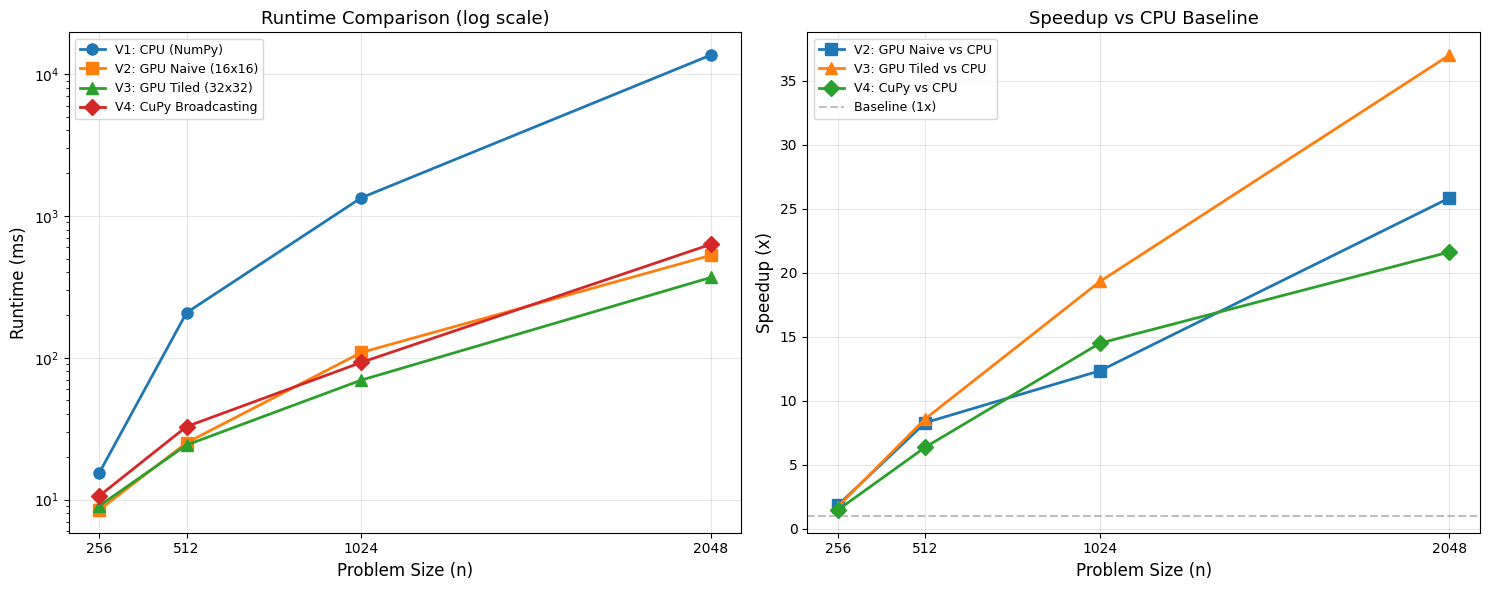
\includegraphics[width=\textwidth]{benchmarks_plottings.png}
\caption{Left: Runtime comparison (log scale). Right: Speedup vs CPU baseline.}
\label{fig:plots}
\end{figure}

\subsection{Left Plot: Runtime Comparison (Log Scale)}

The left plot shows wall-clock runtime (ms, log scale) versus problem size $n$ for all four variants.

\begin{itemize}
  \item The \textbf{CPU line (blue circles)} is consistently the highest, showing it is the slowest variant at every size. Its runtime grows steeply --- from 15.4 ms at $n = 256$ to 13,607.6 ms at $n = 2048$ --- reflecting the $O(n^3)$ complexity running on a single core.

  \item At \textbf{$n = 256$}, all four variants are clustered together (8--15 ms). The GPU variants are only marginally faster because the matrix is too small (65,536 cells) to fully utilize the Tesla T4's 2,560 CUDA cores. Kernel launch overhead and data transfer dominate at this size.

  \item Starting at \textbf{$n = 512$}, the GPU variants clearly separate from CPU. The gap widens dramatically at $n = 1024$ and $n = 2048$, where the GPU has enough parallel work ($n^2$ cells per kernel) to stay busy.

  \item The \textbf{tiled kernel (green triangles)} is the fastest line from $n = 1024$ onward, pulling below both the naive kernel and CuPy. At $n = 2048$, tiled finishes in 367.9 ms versus 526.9 ms for naive --- a clear separation visible on the plot.

  \item \textbf{CuPy (red diamonds)} and \textbf{naive (orange squares)} trade positions. CuPy is slightly slower than naive at small sizes but competitive at $n = 1024$. At $n = 2048$, CuPy is actually the slowest GPU variant (629.9 ms), likely due to the overhead of launching multiple internal kernels per $k$-step.
\end{itemize}

\subsection{Right Plot: Speedup vs CPU Baseline}

The right plot shows speedup (CPU time / GPU time) for the three GPU variants. Higher is better; the gray dashed line at $1\times$ represents the CPU baseline.

\begin{itemize}
  \item At \textbf{$n = 256$}, all GPU speedups are modest (1.45--1.82$\times$). The GPU barely outperforms the CPU because the problem is too small.

  \item Speedups grow steadily with $n$. At \textbf{$n = 512$}, all three GPU variants achieve 6--8$\times$ speedup.

  \item At \textbf{$n = 1024$}, the tiled kernel pulls ahead with \textbf{19.30$\times$} speedup, while naive achieves 12.33$\times$ and CuPy achieves 14.48$\times$. This is where shared-memory tiling starts paying off significantly.

  \item At \textbf{$n = 2048$}, the tiled kernel reaches \textbf{36.99$\times$} speedup --- the highest of all variants. The naive kernel achieves 25.83$\times$ and CuPy achieves 21.60$\times$. The tiled kernel is 1.43$\times$ faster than the naive kernel at this size.

  \item The \textbf{tiled-vs-naive gap widens} with $n$: from 0.94$\times$ at $n = 256$ (tiled was actually slightly slower) to 1.57$\times$ at $n = 1024$ and 1.43$\times$ at $n = 2048$. This confirms that shared-memory optimization becomes more impactful as the matrix grows and there are more redundant global memory reads to eliminate.
\end{itemize}

% ============================================================
\section{What Can Be Inferred from the Results}
% ============================================================

\subsection{CPU vs GPU Baseline (Variant 1 vs Variant 2)}

The naive GPU kernel already provides substantial speedup over the CPU baseline, reaching 25.83$\times$ at $n = 2048$. This makes sense because each $k$-step updates $n^2$ independent cells, and the GPU can process them in parallel across its 2,560 cores. The CPU, limited to a single core with NumPy vectorization, cannot match this level of parallelism.

However, the naive kernel leaves performance on the table because it wastes memory bandwidth on redundant reads.

\subsection{CPU vs Tiled Kernel (Variant 1 vs Variant 3)}

The tiled kernel provides the best overall speedup, reaching 36.99$\times$ at $n = 2048$. Compared to the naive kernel's 25.83$\times$, this is a 43\% additional improvement purely from shared-memory tiling. The benefit grows with problem size because larger matrices generate more blocks, and each block saves more redundant reads.

\subsection{Naive vs Tiled Kernel (Variant 2 vs Variant 3)}

At $n = 256$, the tiled kernel is actually 6\% \emph{slower} than the naive kernel (9.0 ms vs 8.4 ms). This is because the overhead of shared-memory loading and \texttt{syncthreads()} outweighs the benefit when the matrix is small and there are few blocks. But by $n = 1024$, the tiled kernel is 1.57$\times$ faster, and at $n = 2048$ it is 1.43$\times$ faster. The shared-memory optimization clearly pays off at scale.

\subsection{CuPy vs Hand-Written Kernels (Variant 4 vs Variants 2/3)}

CuPy's performance is mixed. At $n = 1024$, CuPy (92.6 ms) is actually faster than the naive kernel (108.8 ms), suggesting that CuPy's internal kernels are well-optimized. But at $n = 2048$, CuPy (629.9 ms) is the slowest GPU variant, slower than even the naive kernel (526.9 ms). This is likely because at large $n$, the per-$k$ overhead of launching multiple CuPy kernels (slicing + addition + minimum) accumulates significantly across 2048 iterations.

CuPy demonstrates a practical tradeoff: it is much easier to write and debug than hand-written CUDA kernels, but gives up control over memory hierarchy and kernel launch patterns.

% ============================================================
\section{Bottleneck Analysis}
% ============================================================

\subsection{Memory Traffic vs Arithmetic}

Floyd--Warshall has very low arithmetic intensity. Each cell update involves:
\begin{itemize}
  \item 1 addition (\texttt{D[i][k] + D[k][j]}) and 1 comparison (\texttt{min}) = 2 FLOPs
  \item 3 memory reads (\texttt{D[i][j]}, \texttt{D[i][k]}, \texttt{D[k][j]}) = 12 bytes
  \item 1 conditional write (\texttt{D[i][j]}) = 4 bytes
\end{itemize}

That gives an arithmetic intensity of roughly $\frac{2 \text{ FLOPs}}{12 \text{ bytes}} \approx 0.17$ FLOP/byte. The Tesla T4 has a compute-to-bandwidth ratio of roughly 65 FLOP/byte for FP32. This means Floyd--Warshall is \textbf{heavily memory-bandwidth bound} --- the GPU cores sit idle most of the time waiting for data from global memory. Our measured CPU throughput of 1.26--2.18 GFLOP/s (far below the CPU's theoretical peak) confirms this.

\subsection{How the Naive ``One Thread per (i,j) per k'' Design Limits Performance}

The naive kernel in R1 (lines 64--82) and R2 (cell 5) has three specific limitations visible in our results:

\begin{enumerate}
  \item \textbf{Redundant global memory reads:} In our Variant 2 kernel (Cell 3, lines 5--6 of \texttt{naive\_floyd\_kernel}), every thread independently fetches \texttt{dist\_matrix[i, k]} and \texttt{dist\_matrix[k, j]} from global memory. Within a $16 \times 16$ block, 256 threads generate 512 global reads for just 32 unique values. This directly explains why the tiled kernel (Cell 4, which caches these values in shared memory on lines 12--15) is 1.43--1.57$\times$ faster at large $n$.

  \item \textbf{One kernel launch per $k$:} In our Variant 2 wrapper (Cell 3, \texttt{floyd\_warshall\_gpu\_naive}), the host-side loop launches $n$ separate kernels:
\begin{lstlisting}[language=Python]
for k in range(num_nodes):
    naive_floyd_kernel[blocks_per_grid, threads_per_block](
        dist_device, num_nodes, k)
\end{lstlisting}
At $n = 2048$, that is 2,048 launches, each with setup and synchronization overhead. CuPy (Cell 5) has even more overhead --- each $k$ iteration launches multiple internal kernels for slicing, addition, and \texttt{cp.minimum}.

  \item \textbf{Small block size:} The $16 \times 16$ block in Variant 2 (Cell 3, \texttt{threads\_per\_block = (16, 16)}) uses only 256 of the maximum 1,024 threads per block, potentially underutilizing the GPU's streaming multiprocessors. Our tiled kernel (Cell 4) uses \texttt{TILE\_SIZE = 32}, giving $32 \times 32 = 1{,}024$ threads per block --- the CUDA maximum.
\end{enumerate}

\subsection{How Our Changes Address These Issues}

\textbf{Variant 3 (tiled kernel, Cell 4)} directly addresses limitation 1 by loading row $k$ and column $k$ into \texttt{shared\_row\_k} and \texttt{shared\_col\_k} arrays (lines 3--4 of \texttt{tiled\_floyd\_kernel}), then reading from them on lines 20--21. It also addresses limitation 3 with \texttt{TILE\_SIZE = 32}, giving a larger $32 \times 32$ block. The result: 36.99$\times$ speedup vs CPU at $n = 2048$, compared to 25.83$\times$ for the naive kernel.

\textbf{Variant 4 (CuPy, Cell 5)} addresses code complexity --- \texttt{floyd\_warshall\_cupy} is 12 lines of code versus 40+ for the Numba kernels. CuPy's internal kernels may use optimizations we do not have access to, which explains its strong performance at $n = 1024$. However, the per-$k$ kernel launch overhead from \texttt{cp.minimum} (line 9) limits it at $n = 2048$.

% ============================================================
\section{Proposed Further Enhancements}
% ============================================================

Based on the bottlenecks identified above, the following enhancements would further improve performance:

\subsection{3-Phase Blocked Floyd--Warshall}

Our tiled kernel caches row $k$ and column $k$ per block, but still launches one kernel per $k$. A full blocked algorithm would divide the matrix into $B \times B$ tiles and process each $k$-step in three phases:

\begin{enumerate}
  \item \textbf{Phase 1 -- Pivot tile:} Update the tile containing row $k$ and column $k$. It depends only on itself and can be processed entirely in shared memory.
  \item \textbf{Phase 2 -- Cross tiles:} Update tiles in the same row/column as the pivot. Each depends on the pivot tile's results.
  \item \textbf{Phase 3 -- Remaining tiles:} Update all other tiles, each depending on one row-cross and one column-cross tile.
\end{enumerate}

This keeps data in shared memory across multiple $k$-steps within a tile, further reducing global memory traffic. Research has shown 5--10$\times$ speedup over naive kernels on large matrices.

\subsection{PCAM-Style 2D Block Decomposition}

Following Quinn's Chapter 6 methodology, a richer decomposition would partition the matrix into 2D blocks and assign each to a processing unit. Communication would involve exchanging pivot tiles at each $k$-step rather than entire rows and columns, which is more efficient for large processor counts.

\subsection{Multi-GPU Distribution}

For very large graphs ($n > 10{,}000$), the matrix may not fit in a single GPU's 16 GB memory. A natural extension is to distribute the matrix across multiple GPUs using a 1D row or 2D block decomposition. At each $k$-step, the GPU owning row $k$ broadcasts it to all others. With NVLink or CUDA-aware MPI, this communication can be overlapped with computation on non-$k$ rows.

% ============================================================
\section{Modern Context}
% ============================================================

\subsection{When to Use Floyd--Warshall vs Alternatives}

Floyd--Warshall is best suited for \textbf{dense graphs} where most node pairs have edges. Its $O(n^3)$ complexity does not depend on the number of edges. For sparse graphs, running Dijkstra's algorithm from each source ($O(n \cdot E \log n)$) is more efficient. In practice, Floyd--Warshall remains relevant for network routing tables, transitive closure, and dense graph analytics where the all-pairs shortest path matrix is needed.

% ============================================================
\section{Conclusion}
% ============================================================

Starting from R2's reference implementations, I built two modernized GPU variants. The shared-memory tiled kernel (Variant 3) achieved the best performance at every large problem size, reaching \textbf{36.99$\times$} speedup over the CPU baseline at $n = 2048$ and \textbf{1.43$\times$} improvement over the naive GPU kernel. The CuPy broadcasting variant (Variant 4) demonstrated that high-level GPU programming can be competitive (14.48$\times$ at $n = 1024$) while requiring far less code, though it struggles at very large sizes due to kernel launch overhead. The results confirm that Floyd--Warshall is memory-bandwidth bound, and that shared-memory tiling is an effective optimization for reducing redundant global memory traffic on GPUs. Further gains would come from a full 3-phase blocked algorithm and multi-GPU distribution.

% ============================================================
\section{Video Recording}
% ============================================================

The 10-minute walkthrough recording for Part 3 (Track A) can be accessed at the following link:

\url{https://myharrisburgu-my.sharepoint.com/:v:/g/personal/kfernandes_my_harrisburgu_edu/IQCV7EVDJVGeRohjBfbMxT8hAUTspwo_Blqf_85ye0_dY7Y}

\end{document}
